\chapter{Data Analysis}

The aforementioned surveys and interviews yielded a total of \participantCount{} survey responses and one in-depth interviews. The following sections delineate the analytical methodologies employed to scrutinize the data obtained from these surveys and interviews.

\section{Analysis of Multiple-Choice Questions}
\label{sec:pls-sem}

\subsection{Introduction}

Data analysis is a critical component of research across various domains, providing essential insights and driving informed decision-making. As data complexity and volume continue to grow, so does the need for sophisticated techniques to analyze and interpret this data effectively. This section explores several prominent data analysis techniques used in contemporary research, followed by an in-depth discussion of Partial Least Squares Structural Equation Modeling (PLS-SEM). We will conclude with a rationale for choosing PLS-SEM as the most suitable method for our thesis. 

\subsection{Data Analysis Techniques}

The field of data analysis encompasses a wide range of techniques and methods designed to extract meaningful insights from complex datasets. These techniques serve various analytical purposes, from understanding fundamental patterns in data to developing sophisticated predictive models. Given the diversity of data types, research objectives, and contexts in which data is analyzed, selecting the appropriate method is crucial for achieving reliable and valid results. This section provides a concise overview of several key data analysis techniques commonly employed in academic and professional research. Each method offers unique advantages and is suited to specific types of data and research questions, contributing to the robust analysis and interpretation of data in various domains.

\hfill \\


\begin{description}[font=\normalfont\itshape]
    \item[\textit{\textbf{Descriptive Statistics}}] Descriptive statistics provide a foundational understanding of data by summarizing its main characteristics through measures such as mean, median, mode, and standard deviation. These statistics are essential for preliminary data analysis, offering a snapshot of data distribution and variability \parencite{Mann2018IntroductoryStatistics}.

    \item[\textit{\textbf{Regression Analysis}}] Regression analysis is a powerful technique used to understand the relationship between dependent and independent variables. It includes various forms such as linear regression, logistic regression, and multiple regression, each serving specific analytical needs \parencite{Montgomery2021IntroductionAnalysis}.

    \item[\textit{\textbf{Factor Analysis}}] Factor analysis is used to identify underlying relationships between measured variables. It helps in data reduction by grouping variables into factors based on their correlations, making complex data more manageable and interpretable \parencite{Andy2018DiscoveringStatistics}.

    \item[\textit{\textbf{Cluster Analysis}}] Cluster analysis involves grouping a set of objects in such a way that objects in the same group (or cluster) are more similar to each other than to those in other groups. This technique is widely used in market research, pattern recognition, and bioinformatics \parencite{Hair2019WhenPLS-SEM}.

    \item[\textit{\textbf{Time Series Analysis}}] Time series analysis focuses on analyzing data points collected or recorded at specific time intervals. Techniques such as ARIMA and Exponential Smoothing are used to forecast future trends based on historical data \parencite{Box2015TimeControl}.

    \item[\textit{\textbf{Partial Least Squares Structural Equation Modeling (PLS-SEM)}}] \hfill \\
    PLS-SEM is a multivariate statistical analysis technique used to analyze complex relationships among variables. It is particularly useful for predictive modeling and theory building in situations where the data is not normally distributed or the sample size is small \parencite{Sarstedt2017PartialModeling}.
\end{description}


\subsection{PLS SEM for Research}

Partial Least Squares Structural Equation Modeling (PLS-SEM) is a powerful statistical technique and a second-generation multivariate method gaining traction in various research fields, particularly in social sciences, business research, marketing, and information systems. It allows researchers to construct and test complex models involving multiple latent and observed variables and is particularly useful for models with numerous variables, intricate relationships, and multiple indicators for each variable \parencite{Sarstedt2017PartialModeling, Henseler2015AModeling}. PLS-SEM helps researchers analyze the interplay between multiple variables, including those not directly measurable (latent variables), thereby providing a deeper understanding of cause-and-effect relationships in complex systems \parencite{Sarstedt2017PartialModeling}. Unlike Covariance-Based SEM (CB-SEM), PLS-SEM focuses on maximizing the explained variance of dependent constructs, making it an ideal choice for predictive modeling, theory development, and exploratory research \parencite{Chin1998TheModeling} \parencite{Sarstedt2017PartialModeling}. In contrast to techniques focused on confirming existing theories, PLS-SEM is particularly suited for developing new theories or extending existing ones, especially when the goal is to predict or identify key factors influencing a phenomenon \parencite{Chin1998TheModeling}. PLS-SEM thrives in contexts where data complexity is the norm, such as in studying intricate systems like family businesses or large-scale marketing campaigns \parencite{Henseler2015AModeling}. PLS-SEM's robustness and flexibility allow it to handle challenging data conditions that traditional methods may not manage effectively. It accommodates both reflective and formative measurement approaches, offering the flexibility to choose between indicators that either reflect or form the underlying concept, depending on the research question \parencite{Chin1998TheModeling}. This method is advantageous in dealing with real-world data that does not always follow a perfect normal distribution, making minimal assumptions about the underlying data distribution \parencite{Lohmoller1989LatentSquares}. It also supports the evaluation of theoretical models, even with smaller sample sizes, unlike other techniques that require larger samples for accuracy \parencite{Sarstedt2017PartialModeling}. The methodology has gained popularity in fields such as marketing, information systems, and social sciences due to its capacity to model intricate relationships and assess the reliability and validity of constructs, even with small samples and non-normal data distributions \parencite{Chin1998TheModeling}. It effectively tackles common challenges in social science research, making it particularly suitable for complex models where data may be limited or challenging to collect. Moreover, PLS-SEM has been highlighted as a robust solution in evaluating theoretical models in the social sciences, business research, and other fields where data complexity is prevalent \parencite{Sarstedt2017PartialModeling}.

PLS-SEM is well-suited for exploratory research and prediction-oriented studies due to its focus on maximizing the explained variance of the dependent variables \parencite{Henseler2015AModeling}. Unlike traditional covariance-based SEM methods, which often require larger sample sizes and confirmatory analysis, PLS-SEM provides a reliable alternative for research scenarios that demand flexibility and adaptability in dealing with diverse data structures and research objectives.

\subsubsection{Key Features of PLS-SEM}

PLS-SEM prioritizes prediction, making it suitable for exploratory research where theory is less developed.It is capable of handling both reflective and formative measurement models \parencite{Chin1998TheModeling}. It is effective with small to medium sample sizes, which is often a limitation in other SEM approaches \parencite{Sarstedt2017PartialModeling}. It is robust against deviations from normality, allowing for broader applicability across different datasets \parencite{Henseler2015AModeling}. Additionally, PLS-SEM offers a valuable toolkit for researchers navigating complex relationships and data limitations. Its ability to handle intricate models, work with small samples, and provide flexibility in measurement makes it a compelling choice for various research endeavors \parencite{Tenenhaus2005PLSModeling}.

\subsubsection{Steps in PLS-SEM}

\begin{itemize}
    \item \textbf{Model Specification}: Define the structural and measurement models. The structural model (inner model) specifies relationships between latent variables, while the measurement model (outer model) links latent variables to their indicators \parencite{Lohmoller1989LatentSquares}.

    \item \textbf{Model Identification}: Ensure the model is identified with sufficient data points to estimate parameters.

    \item \textbf{Data Collection}: Gather data for all observed variables.

    \item \textbf{Model Estimation}: Use the PLS algorithm to estimate path coefficients, weights, and loadings \parencite{Wold1985SystemsSquares}.

    \item \textbf{Model Evaluation}: Assess the model using criteria such as convergent validity, discriminant validity, composite reliability, and R² values \parencite{Tenenhaus2005PLSModeling}.

    \item \textbf{Model Interpretation}: Interpret the results to draw meaningful conclusions about the relationships between constructs.
\end{itemize}

\subsubsection{Model Evaluation Criteria}

\begin{itemize}
    \item \textbf{Convergent Validity}: Assessed through Average Variance Extracted (AVE), which should exceed 0.50 \parencite{Henseler2015AModeling}.

    \item \textbf{Discriminant Validity}: Evaluated using the Fornell-Larcker criterion, where the AVE of each construct should be greater than the squared correlations with other constructs \parencite{Henseler2015AModeling}.

    \item \textbf{Composite Reliability}: Should be above 0.70 to ensure reliability of constructs \parencite{Sarstedt2017PartialModeling}.

    \item \textbf{R\textsuperscript{2} Values}: Indicate the amount of variance in the dependent variables explained by the model.
\end{itemize}

\subsubsection{Motivation for Using PLS-SEM}

The choice of PLS-SEM for our research is motivated by several factors:

\textbf{1. Handling Complex Models:} Our research involves complex models with multiple constructs and indicators, making PLS-SEM an ideal choice due to its ability to handle such complexity efficiently.

\textbf{2. Predictive Accuracy:} PLS-SEM focuses on maximizing the explained variance, providing better predictive accuracy, which is crucial for our study's objectives.

\textbf{3. Robustness to Data Issues:} PLS-SEM is robust to deviations from normality and can work effectively with small sample sizes, addressing potential limitations in our dataset.

\textbf{4. Theory Development and Validation:} Given that our research aims to both develop and validate theoretical models, PLS-SEM offers the necessary tools for rigorous analysis and validation.

In conclusion, PLS-SEM offers a valuable toolkit for researchers navigating complex relationships and data limitations. Its ability to handle intricate models, work with small samples, and provide flexibility in measurement makes it a compelling choice for various research endeavors \parencite{Tenenhaus2005PLSModeling}.


% \textbf{Application of PLS-SEM} 

% Having developed the constructs and hypotheses, we will now apply PLS-SEM to analyze the data collected from the responses to questions 4-10. This analysis will involve the following steps: 

% \textbf{1. Model Specification:} 

% Define the relationships between constructs and indicators. Specify the hypothesized relationships among the constructs. 

% \textbf{2. Data Collection and Preparation:} 

% Gather responses to the selected questions. Prepare the data for analysis, ensuring it meets the requirements for PLS-SEM. 

% \textbf{3. Model Estimation:} 

% Use PLS-SEM software to estimate the model parameters. Assess the measurement model for reliability and validity. 

% \textbf{4. Structural Model Evaluation:} 

% Evaluate the structural model by examining path coefficients and the significance of hypothesized relationships. Assess the model’s explanatory power through measures such as R-squared and Q-squared statistics. 

% \textbf{5. Hypothesis Testing: }

 

% Test the formulated hypotheses using the results from the structural model evaluation. Validate or invalidate each hypothesis based on the significance and direction of the relationships. Through this systematic application of PLS-SEM, we aim to derive meaningful insights from our data and validate the proposed hypotheses, thereby advancing our understanding of the impact of pandemic disruptions on change management and resilience strategies. 

\subsection{Application of PLS-SEM}

In our study, we utilized SmartPLS 4 \parencite{smartpls2024} to analyze the structural equation model (SEM) based on the survey data collected. The constructs and hypotheses were operationalized through a series of survey questions, each carefully designed to measure specific aspects of the constructs in question. Below, we will elaborate on the process of model construction and the rationale behind the arrows and dependencies depicted in the Figure \ref{fig:constructs}. The survey data comprised questions targeted at measuring three main constructs: Pandemic Disruption, Change Management, and Resilience Effectiveness. Each of these constructs was associated with specific questions from the survey. For Pandemic Disruption, we used Question 4 which assesses the extent to which companies experienced supply chain disruptions due to the pandemic. This question serves as a critical indicator of the impact of COVID-19 on operational stability. Change Management was measured using Questions 5, 6, 8, 9, and 10. These questions capture various strategic responses implemented during the pandemic, including changes in supply management strategies, supplier diversification, creation of backup plans, adjustment of demand forecasting methods, and the presence of formal pandemic preparedness plans. These aspects collectively reflect the strategic adaptability and preparedness measures undertaken by companies in response to the pandemic. Resilience Effectiveness was gauged through Question 7, which evaluates the effectiveness of the company's resilience strategies such as inventory management and supplier diversification during the pandemic. This construct provides insights into how well existing strategies mitigated the pandemic's impact. The diagram also incorporates the specific survey questions associated with each construct, denoted by the yellow text boxes. For example, CMQ10, CMQ5, CMQ6, CMQ8, and CMQ9 represent the questions related to Change Management. The arrows pointing towards the Change Management node indicate the reflective measurement model, where each question (indicator) is influenced by the underlying construct. PLS-SEM analysis is well suited for various types of research data, some of them being the Likert Scale, which typically is a 5-point scale where respondents indicate their level of agreement or disagreement with a statement. The scales usually range from "Strongly Agree" to "Strongly Disagree", or similar. Likert scales are popular in measuring attitudes, perceptions, and behavioral intentions. It is also suited for Binary or Dichotomous Scales, which are simple yes/no or true/false responses. In our case, the responses for Questions 4 and 7 are in the Likert Scale and the responses for Questions 5, 6, 8, 9 and 10 are within the Binary Scale. This is briefly below.

\subsubsection{Methodology Steps}

\paragraph*{Selection of Questions for Analysis:} To apply PLS-SEM, we selected questions 4 to 10 for analysis. These questions were chosen because they are either yes/no questions or questions with answers on a scale ranging from 0 to 5, which are suitable for the PLS-SEM modeling approach.

\paragraph*{Construct Development:} To create meaningful hypotheses, constructs are developed based on the questions asked, specifically questions 4-10. Constructs represent the theoretical concepts that underpin the variables of interest in the study.

\paragraph*{Hypothesis Creation and Validation:} The primary objective is to formulate hypotheses based on the research questions and subsequently validate or invalidate them using the responses received. The validation will be conducted through the results obtained from the PLS-SEM analysis.

\paragraph*{Summary of Process:}

\begin{itemize}
    \item \textbf{Step 1:} Select objective questions (Questions 4-10).
    \item \textbf{Step 2:} Develop constructs based on the selected questions.
    \item \textbf{Step 3:} Formulate hypotheses related to the developed constructs.
    \item \textbf{Step 4:} Apply PLS-SEM to analyze the data and obtain results.
    \item \textbf{Step 5:} Validate or invalidate the hypotheses based on the analysis results.
\end{itemize}

\subsubsection{Constructs Developed}

\paragraph*{Construct 1: Pandemic Disruption}

\begin{itemize}
    \item \textbf{Question Used:} Question 4
    \item This construct is based on a question that measures the extent to which companies experienced disruption in their supply chain due to the pandemic. It serves as an indicator of the overall impact of COVID-19 on operations.
\end{itemize}

\paragraph*{Construct 2: Change Management}

\begin{itemize}
    \item \textbf{Questions Used:} Questions 5, 6, 8, 9, 10
    \item These questions pertain to various changes implemented in response to the pandemic, including adjusting management strategies, diversifying suppliers, creating backup plans, adjusting forecasting methods, and formalizing preparedness plans. These questions reflect the strategic adaptability and preparedness measures taken by companies.
\end{itemize}

\paragraph*{Construct 3: Resilience Effectiveness}

\begin{itemize}
    \item \textbf{Question Used:} Question 7
    \item This construct evaluates the effectiveness of the company’s resilience strategies during the pandemic, such as inventory management and supplier diversification.
\end{itemize}



\begin{figure}[H]
  \centering
  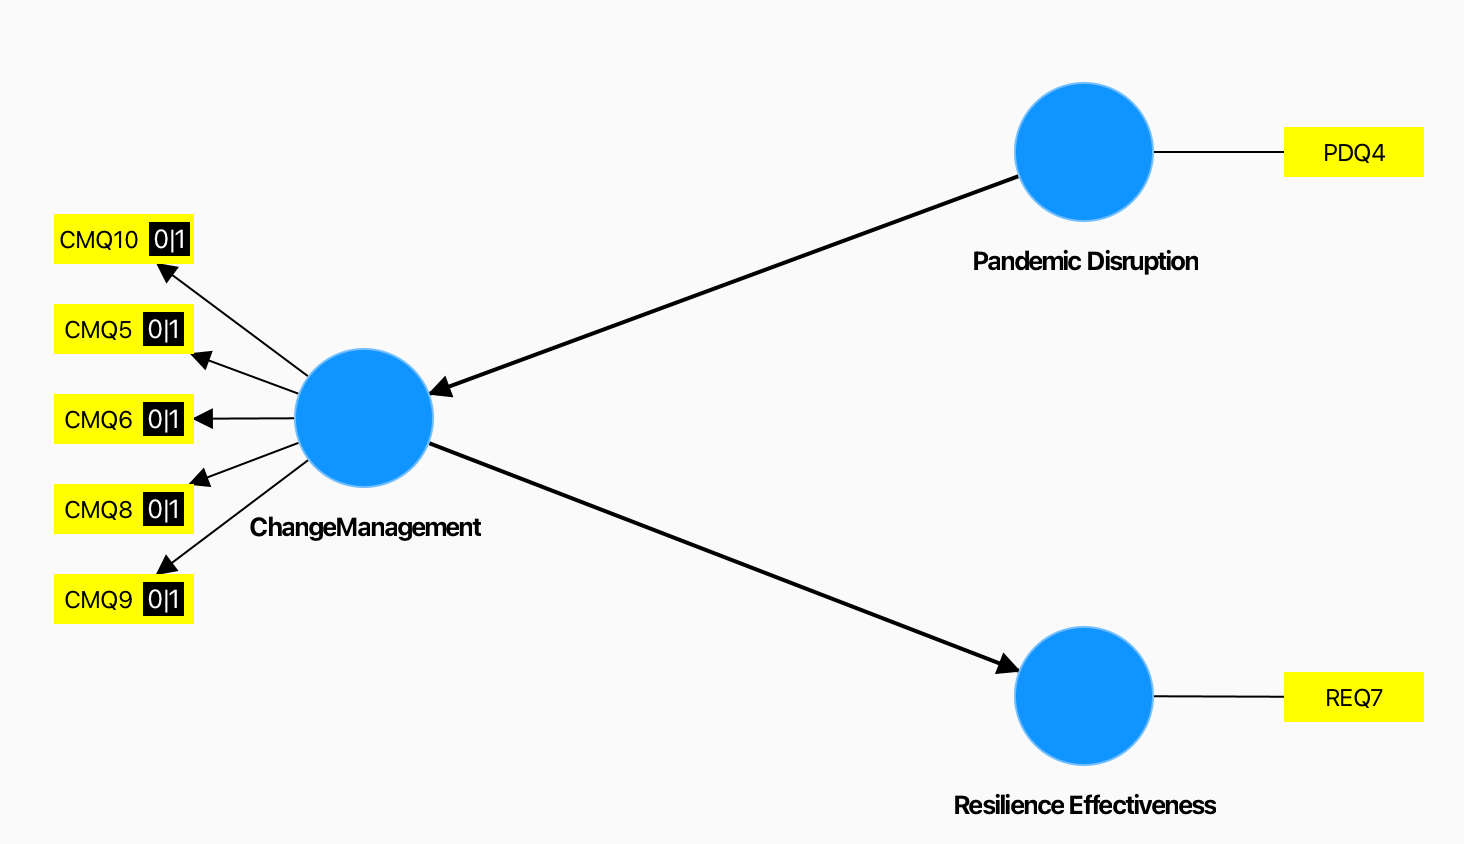
\includegraphics[width=1\textwidth]{figure/initial_model.png}
  \caption{Structural Model in SmartPLS showing the relationships between constructs. The model includes Pandemic Disruption (Q4), Change Management (Q5, Q6, Q8, Q9, 10), and Resilience Effectiveness (Q7). Arrows indicate hypothesized dependencies: Pandemic Disruption's impact on Change Management and Resilience Effectiveness, and Resilience Effectiveness's influence on Change Management. $[0|1]$ Adjacent to the question numbers indicate the binary nature of the questions. Other questions belong to the Likert Scale.}
  \label{fig:constructs}
\end{figure}


Using SmartPLS 4, we constructed a model (Figure \ref{fig:constructs}) to test our hypotheses. The structural model posits the following relationships:

\begin{enumerate}
    \item \textbf{Pandemic Disruption leads to Change Management (H1)}: This hypothesis suggests that higher levels of disruption due to the pandemic are positively associated with an increase in change management strategies. The arrow from Pandemic Disruption to Change Management in the diagram represents this hypothesis. The rationale is that significant disruptions necessitate strategic changes to adapt and mitigate the impact.

    \item \textbf{Resilience Effectiveness reduces the need for extensive Change Management (H2)}: This hypothesis proposes a negative relationship between the effectiveness of resilience strategies and the extent of change management. If a company’s existing resilience strategies are effective, it may not need to implement extensive changes. This is depicted by the arrow from Resilience Effectiveness to Change Management, indicating that effective resilience strategies can mitigate the need for further change.

    \item \textbf{Pandemic Disruption influences Resilience Effectiveness (H3)}: This hypothesis posits a positive relationship between the level of pandemic disruption and the perceived effectiveness of resilience strategies. Higher levels of disruption may prompt companies to evaluate and enhance their resilience strategies, thus leading to higher effectiveness. This relationship is shown by the arrow from Pandemic Disruption to Resilience Effectiveness in the diagram.

\end{enumerate}

Upon conducting the analysis using the SmartPLS tool for PLS-SEM, we can evaluate the validity of our hypothesized relationships among the constructs. By examining the path coefficients, significance levels (p-values), and the R² values for each endogenous construct, SmartPLS provides comprehensive insights into the strength and significance of the proposed causal paths. In our specific case, this involves assessing whether the hypothesized positive relationship between Pandemic Disruption and Change Management, the negative relationship between Resilience Effectiveness and Change Management, and the positive relationship between Pandemic Disruption and Resilience Effectiveness hold true. Additionally, the bootstrapping procedure available in SmartPLS allows us to obtain estimates of standard errors and confidence intervals, further solidifying our hypothesis testing. The evaluation of the model fit indices, such as the SRMR (Standardized Root Mean Square Residual), will help determine the overall adequacy of our model, enabling us to conclude whether the empirical data supports our theoretical propositions. Thus, the detailed results obtained from SmartPLS will enable us to confirm or refute our hypotheses with a considerable degree of statistical confidence. In configuring the SmartPLS software for our PLS-SEM analysis, several key settings were chosen to ensure interpretable results. We selected the Principal Component Analysis (PCA) weighting scheme, a common default choice, as it uses the first principal component of the block’s indicators as the composite score, providing a reliable and standard approach. To facilitate easier interpretation of path coefficients and enable comparisons across constructs, we opted for standardized results, which convert all variables to a common scale. For the initial weights, we adhered to the algorithm’s default settings. Regarding the handling of missing values, considering that only one response was partially missing, we utilized casewise deletion, provided it did not significantly reduce our sample size below acceptable limits for robust analysis. Lastly, we did not apply any additional weighting vectors, as none were necessary for our analysis.

\subsection{Results and Analysis of PLS-SEM}

\begin{figure}[h]
  \centering
  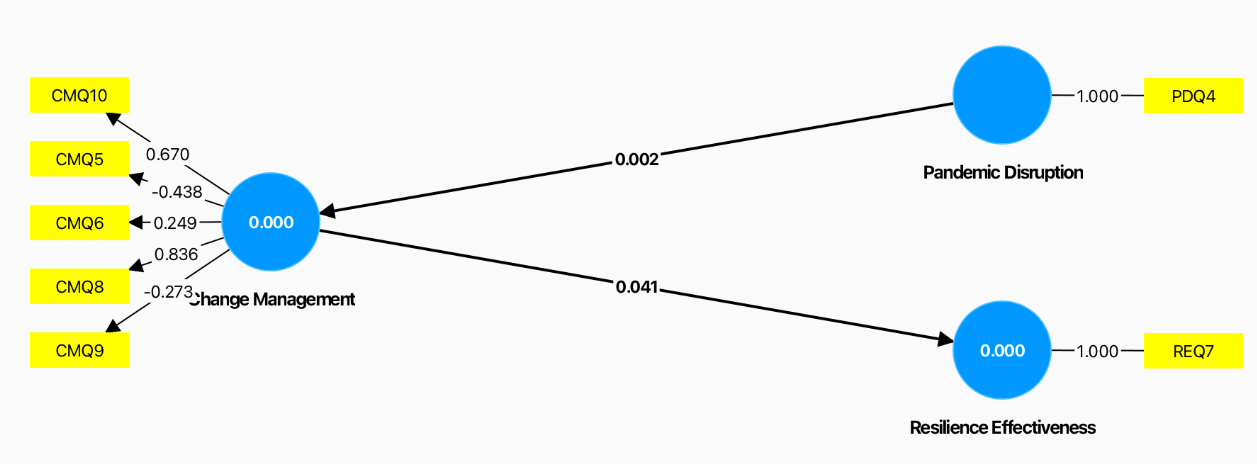
\includegraphics[width=1\textwidth]{figure/pls_sem_results_cropped.png}
  \caption{PLS-SEM Results showcasing path coefficients between constructs.}
  \label{fig:pls_sem_results}
\end{figure}

The results of our PLS-SEM analysis, depicted in Figure \ref{fig:pls_sem_results}, reveal the path coefficients among the constructs of Pandemic Disruption, Change Management, and Resilience Effectiveness. The path coefficient from Pandemic Disruption to Change Management is 0.002, suggesting a minimal positive influence of pandemic-induced disruptions on the extent of change management strategies implemented. This indicates that while pandemic disruptions might necessitate some strategic changes, the direct impact observed here is negligible. Conversely, the path coefficient from Resilience Effectiveness to Change Management is 0.041, implying a slight positive relationship. This suggests that as the effectiveness of resilience strategies increases, there is a marginal but positive impact on change management practices, indicating that companies with effective resilience strategies may still engage in proactive change management. The negative coefficients observed within the Change Management construct, such as -0.438 for CMQ5, -0.249 for CMQ6, and -0.273 for CMQ9, indicate that these specific aspects of change management may inversely relate to the overall construct. This could mean that certain change management practices, possibly those perceived as less effective or unnecessary, might detract from the overall strategic change efforts. The positive coefficients, such as 0.670 for CMQ10 and 0.836 for CMQ8, highlight the aspects that contribute positively to Change Management, signifying effective practices that enhance strategic adaptability. The significant values of 1.000 for PDQ4 and REQ7 indicate strong relationships of these specific questions with their respective constructs, emphasizing their reliability as indicators. Following the discussion on the path coefficients and their implications, we now turn our attention to additional metrics and validity assessments to provide further analysis of the model's performance.

\begin{figure}[h]
  \centering
  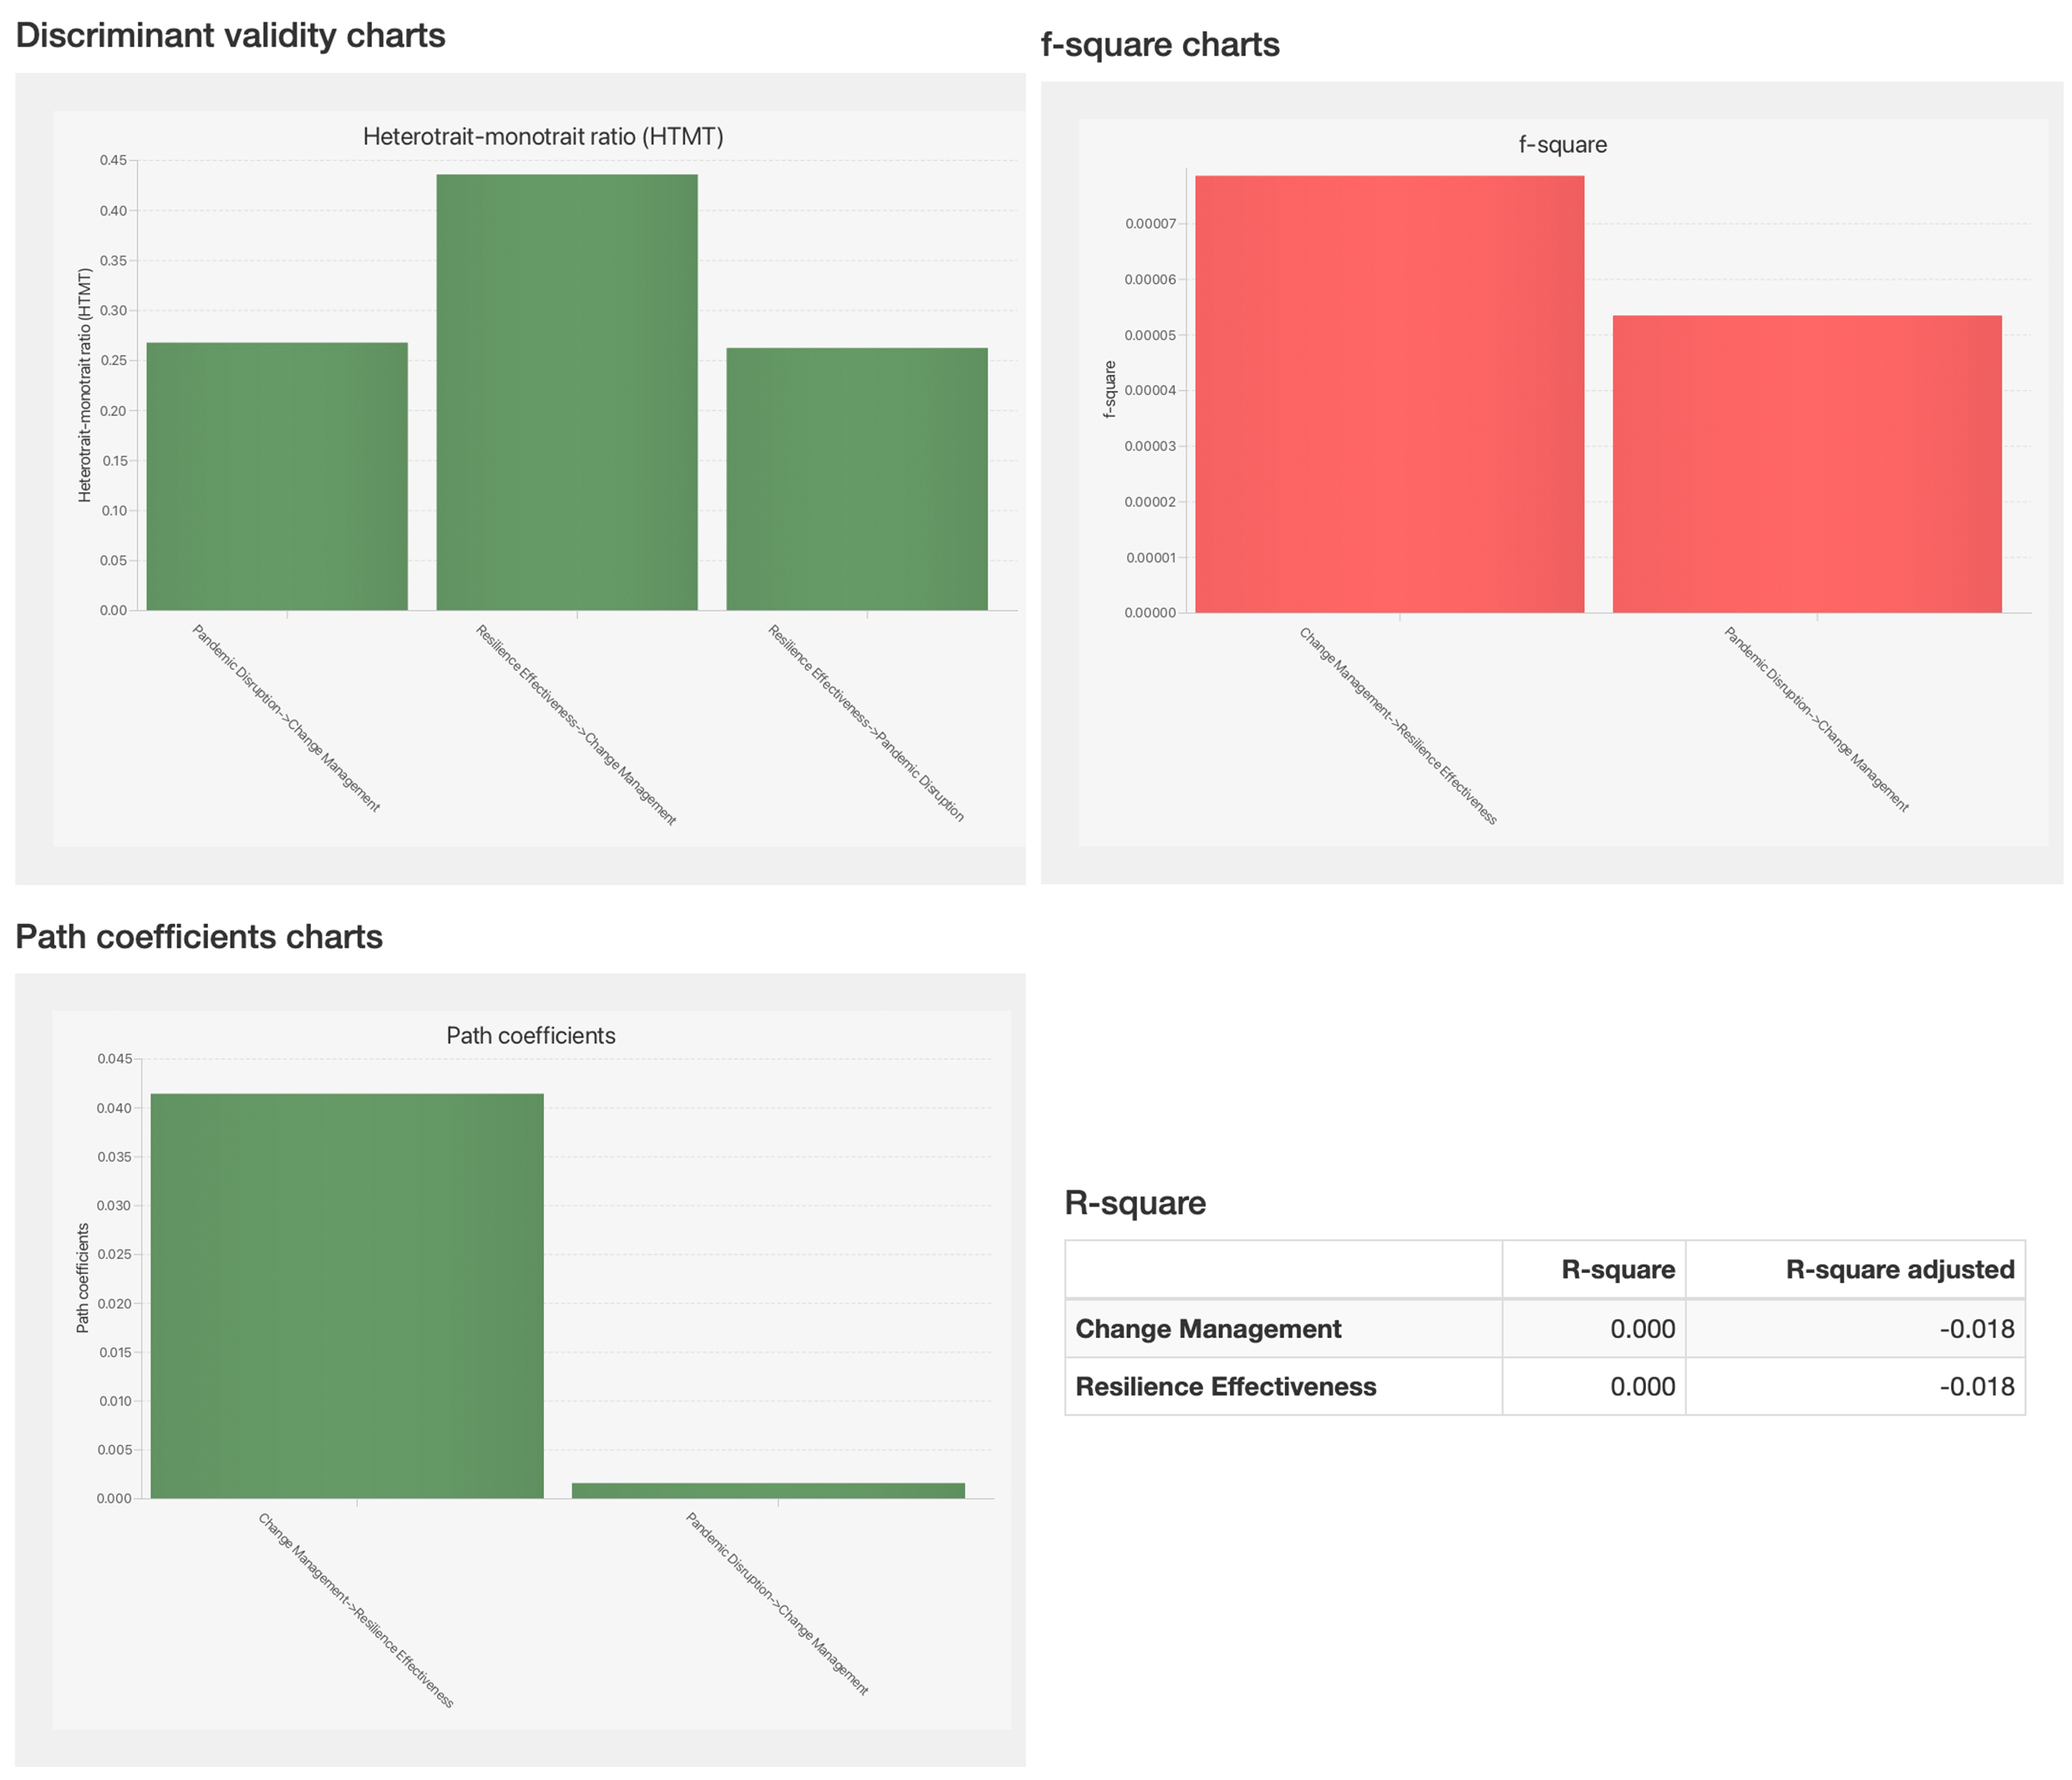
\includegraphics[width=1\textwidth]{figure/other_results.png}
  \caption{Other statistics from PLS-SEM analysis.}
  \label{fig:other_results}
\end{figure}

The results and analysis of PLS-SEM, as depicted in Figure \ref{fig:other_results}, offer further understanding of the relationships between the constructs of Pandemic Disruption, Change Management, and Resilience Effectiveness. The path coefficients chart confirms the previously discussed minimal impact, with the coefficient from Pandemic Disruption to Change Management being virtually zero (0.002), indicating a negligible direct effect. The slightly positive coefficient from Resilience Effectiveness to Change Management (0.041) suggests a weak but positive influence, implying that effective resilience strategies marginally contribute to change management efforts. The R-square values for both Change Management and Resilience Effectiveness are zero, indicating that the model does not explain any variance in these constructs, which may suggest either the lack of a strong relationship or limitations in the model's ability to capture the dynamics. The f-square values, though small, provide insight into the effect sizes, with Change Management to Resilience Effectiveness showing a slightly higher value compared to Pandemic Disruption to Change Management, indicating that resilience strategies have a somewhat more substantial influence on change management. The discriminant validity, assessed through the Heterotrait-Monotrait ratio (HTMT), indicates acceptable values below the threshold of 0.85, confirming that the constructs are distinct from each other. The SRMR (Standardized Root Mean Square Residual) values are 0.172 for the saturated model and 0.180 for the estimated model, both exceeding the recommended threshold of 0.08, suggesting a poor model fit and potential issues with the structural model specification. These results imply that while some relationships are weakly supported, the overall model does not adequately capture the variance and relationships between the constructs, indicating the need for model refinement or consideration of additional variables to better understand the dynamics at play.

Based on expert analysis and observation of our dataset, several factors have been identified that may explain why we were unable to establish strong correlations in our PLS-SEM analysis. Firstly, the lack of variability in the Change Management questions (CMQ5, CMQ6, CMQ8, CMQ9, CMQ10), where responses were predominantly '1' (Yes), significantly limits the statistical power of our analysis. The homogeneity in these responses means there is insufficient variation to explain the variance in dependent constructs, thereby hindering the detection of meaningful relationships. While the Pandemic Disruption variable (PDQ4) exhibited more variability, ranging from 0.8 to 5, its effectiveness in revealing correlations is compromised when paired with less variable indicators. Similarly, Resilience Effectiveness (REQ7) showed reasonable variability, ranging from 1.5 to 5, but the overall analysis suffers from the lack of diversity in binary responses. The binary nature and the high prevalence of a single response category diminish the ability of PLS-SEM to uncover underlying patterns, as significant paths are often established through variance explained by independent variables. The presence of potential ceiling effects, where binary indicators in the Change Management construct consistently hit the upper limit of their scale, further complicates the analysis by obscuring genuine relationships. This effect results in insufficient differentiation among responses, making it difficult to discern how changes in one variable relate to another. Lastly, the model configuration and theoretical considerations play a crucial role; our current model setup may not adequately capture the expected relationships if the theoretical assumptions are not perfectly aligned with the observed data. The predominance of 'yes' responses in the Change Management questions indicates that minor deviations might not statistically explain variations in Resilience Effectiveness, especially if the resilience question encompasses broader aspects of the pandemic's impact than anticipated. Consequently, while the results might indicate no correlation, it is also possible that due to the dataset's characteristics, existing correlations could not be established, highlighting the need for further refinement and consideration of additional variables.
















% \subsubsection{Purpose}
% Placeholder Text

% \subsubsection{Overview}
% Placeholder Text

% \subsection{Model Specification}
% Placeholder Text

% \subsubsection{Constructs and Measurement}
% Placeholder Text

% \subsubsection{Model Design}
% Placeholder Text

% \subsection{Evaluation of Measurement Model}
% Placeholder Text

% \subsubsection{Indicator Reality}
% Placeholder Text

% \subsubsection{Construct Reliability and Validity}
% \textbf{Internal Consistency Reliability}

% \textbf{Convergent Validity}

% \subsubsection{Discriminant Validity}

% \subsubsection{Summary}

% \subsection{Evaluation of Structural Model}

% \subsubsection{Path Analysis}
% \textbf{Path Coefficients}
% \textbf{Direct and Indirect Effects}

% \subsubsection{Model Fit}

% \subsubsection{R-Squared $(R^2)$ Values}

% \subsubsection{Effect Sizes $(f^2)$ Values}

% \subsection{Model Assessment and Validation}

% \subsubsection{Collinearity Statistics}

% \subsubsection{Robustness Checks}

% \subsection{Discussion of Findings}

% \subsubsection{Interpretation of Results}

% \subsubsection{Implications}

% \subsection{Limitations and Future Research Directions}

% \subsection{Conclusion}
\section{Analysis of Open-Ended Responses}
\label{sec:keyword-analysis}

\subsection{Keyword Extraction Process}

As discussed previously, we have introduced one open-ended question within our survey, namely: (Refer the entire questionnaire in Appendix \ref{appendix:survey}).

\begin{tcolorbox}[colback=blue!5!white, colframe=blue!15!black, boxrule=0.5mm, title=Subjective Question, fonttitle=\bfseries]
  We would really appreciate it if you can add some insights based on your personal experience of handling supply chain issues during the pandemic.
\end{tcolorbox}

Due to the nature of this question, a different approach was needed to analyse all the responses. While we have engaged in a thorough qualitative examination of the subjective responses—employing a traditional interpretative approach to manually read and derive inferences from the survey data—our analysis did not stop there. Recognizing the value of quantifiable insights in enhancing the reliability and generalizability of our findings, we subsequently applied statistical methods to analyze these responses. This dual approach enabled us to capture the nuanced perspectives offered by the respondents, and also to quantify patterns and trends that could be systematically validated. In this section we will discuss the quantitative methodology employed by us. 

There are various recognised methodologies that are used to analyse subject data. \textcite{Joshi2024AAnswers} have analysed various methodologies that are used to perform automated assessment for subjective responses as we have received in our questionnaire. Content Analysis \parencite{Harwood2003AnAnalysis}, which is a systematic technique for interpreting textual data by categorizing the content into various groups based on specific criteria. While it can be both qualitative and quantitative, often the frequency of words, phrases or topics are counted to identify patterns or trends. Another prominent methodology, Thematic Analysis \parencite{terry2017thematic} predominantly qualitative and focuses on identifying and analyzing patterns or themes within data. It involves closely reading the text to code data and sort these codes into themes that emerge organically. It's flexible and can uncover rich, detailed, and complex data interpretations. Discourse Analysis \parencite{gill2000discourse}, while defined differently in many literature, generally goes beyond the content of text to consider the context and means of communication. It examines how language is used in the text to convey messages, and how this relates to social and cultural contexts. In addition, another prominent method, Grounded theory \parencite{birks2015grounded_ch1} is used to generate or discover a theory through the data collected. It involves collecting data and analyzing it iteratively. As more data is collected, and analysis proceeds, the emerging theory or conceptual framework starts to take shape. This method is particularly useful for new areas of research where existing theories might not apply. Another prominent methodologies are Sentiment Analysis \parencite{Wankhade2022AChallenges}, Lexical Analysis \parencite{Bolden2000BridgingDivide}, Narrative Analysis \parencite{Burck2005ComparingAnalysis}, Machine Learning Techniques \parencite{Jain2021AReviews, Alantari2022AnReviews} and Keyword Extraction.

Keyword Extraction \parencite{Firoozeh2020KeywordMethods, Bharti2017AutomaticSurvey} is a broad umbrella that includes various automatic and manual methodologies that prominently focuses on extracting keywords from subjective texts. \textcite{Yuan2018TextStrategy} describe some prominent Keyword Extraction algorithms. TF-IDF (Term Frequency-Inverse Document Frequency) is about weighting the frequency of a word in a document against its frequency across all documents to identify its importance, while LDA (Latent Dirichlet Allocation) is a probabilistic model that identifies topics distributed across a corpus of texts and assigns keywords to these topics based on their distribution, furthermore, TextRank is a graph-based ranking model for text processing which forms a network from the text and uses the structure of this network to determine the importance of words or phrases. 

Building on the array of methodologies previously described for analysing textual responses, our approach used in this study diverges somewhat from conventional automated techniques. Insted of deploying established algorithms such as TF-IDF, LDA, or TextRank, we adopted a manual extraction method. This methodological choice was chosen on several key considerations. Firstly, the manageable scope of the dataset - comprising of \participantCount{} responses, each encapsulated within two to three sentences - rendered manual analysis both feasible and practical. This hands-on approach ensured we understand the overall theme of the response, and that we can perform nuanced comprehension and interpretation, which could easily be missed by employing any simple text parsing or word frequency analysis tools/algorithms. For instance, different respondents might articulate similar sentiments or ideas using disparate linguistic expressions, something that purely automated systems could potentially overlook. This manual method, could possibly be categorised, or partially categorised under various analytical paradigms. It shares affinities with \textit{content analysis} in its meticulous parsing of text to identify key terms; and with \textit{thematic analysis} in its sensitivity to underlying themes conveyed across all responses. This technique, however, does not align strictly with any single established methodology like \textit{sentiment analysis} or \textit{discourse analysis}, although it incorporates elements of these through its interpretative elements. The decision to abstain from fully automated methods was also taken due to the desire to preserve the integrity and depth of qualitative data, ensuring that the richness of the respondents' expressions was fully captured and reflected in the analysis. 

In our approach of keyword extraction, our methodology entailed a meticulous manual review of each response. We initiated this process by reading through the first entry comprehensively, extracting prominent keywords that capture the the essence of the respondents' perspectives. Some noteworthy keywords involve "\textit{diversified supplier base}", "\textit{demand forecasting}" and "\textit{strengthening supply ties}". This will be discussed in detail in further sections. It is important to note that the response need not contain the exact phrase of \textit{diversified supplier base}; however, if the respondent talks about diversifying their supplier base in any other way, we have used the a common and popular term that could explain their sentiments in our extraction. The same process is employed in extraction any other keywords from the answer. Subsequent to this extraction, we engage in an iterative review process, where we similarly analyse the next response. If this response discusses something that aligns with any of the existing keywords, we increase the frequency of those keywords by one, meanwhile also trying to extract any more prominent keywords from the response. We keep doing it for all \participantCount{} responses and thus, end up with a list of keywords and their frequencies. Note that the entire process is performed manually by reading through each responses. Eventually, from the list of all available keywords, most frequent keywords are th
en chosen for any further analysis. Figure \ref{fig:kye_extraction} diagrammatically describes the entire keyword extraction process used.

\begin{figure}[ht]
  \centering
  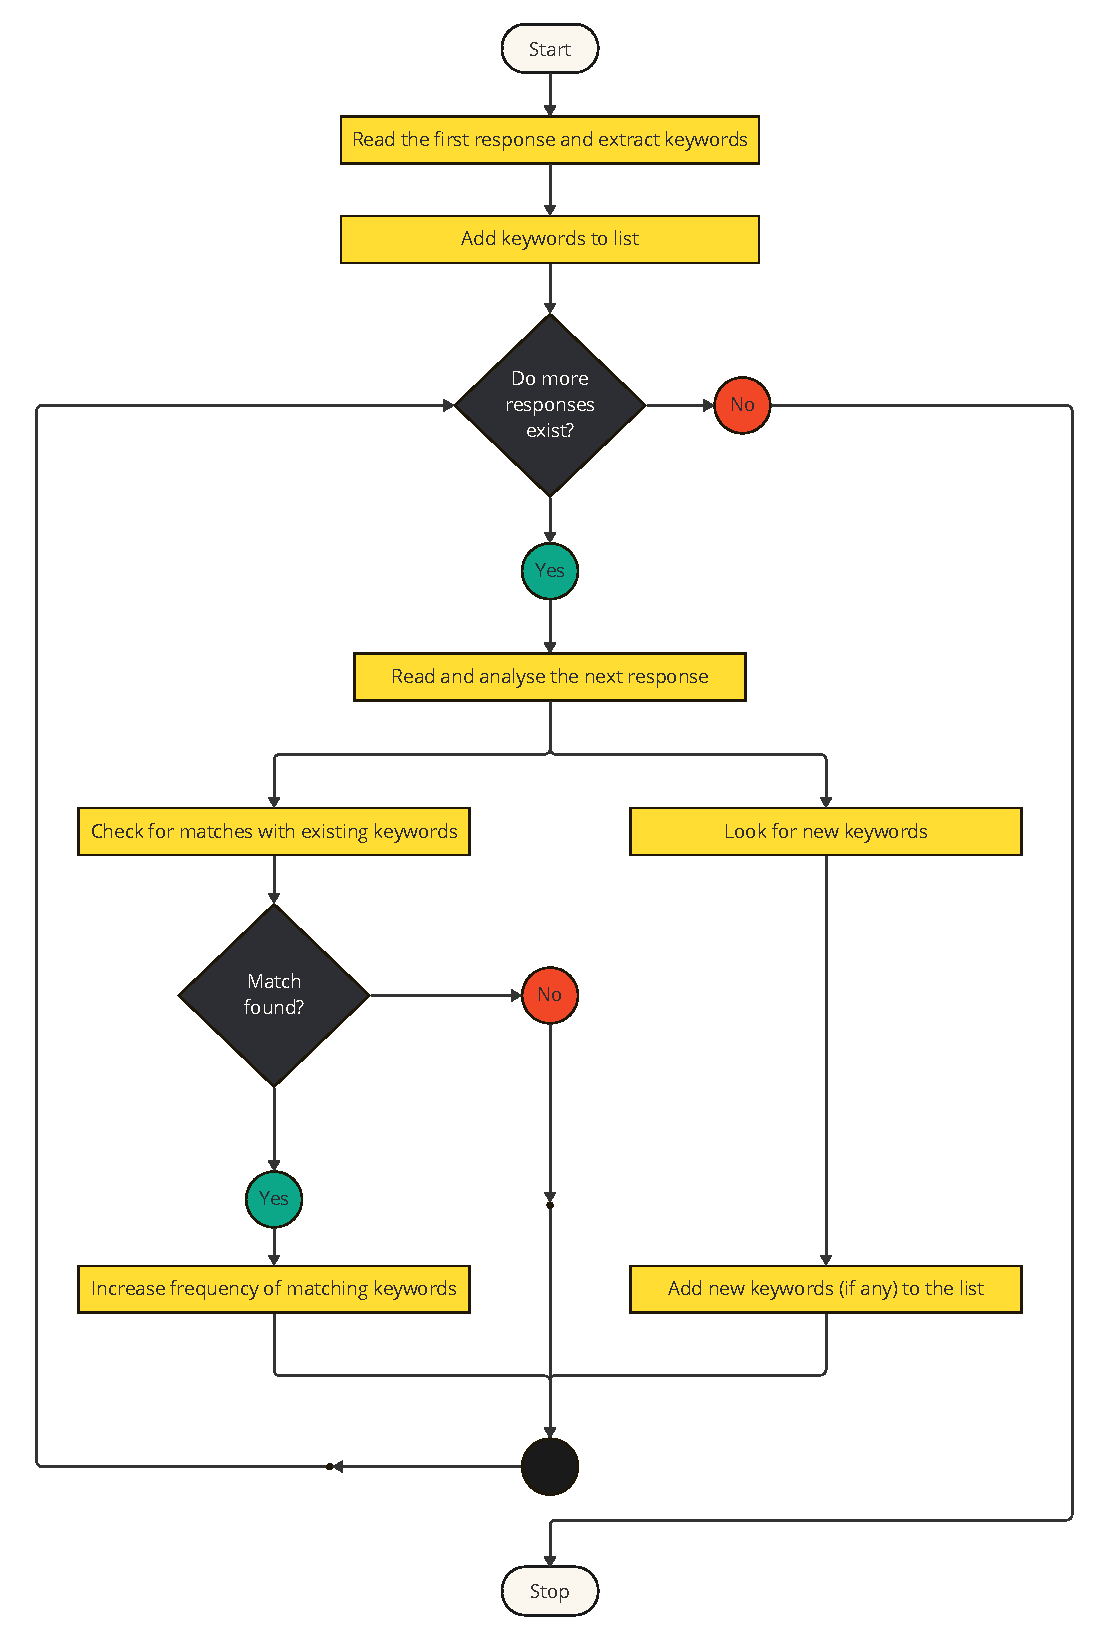
\includegraphics[width=0.6\textwidth]{figure/keyword_extraction_flowchart.pdf}
  \caption{Flowchart of the keyword extraction methodology employed.}
  \label{fig:kye_extraction}
\end{figure}

\subsection{Keyword Analysis}
The analysis resulted in 10 keywords which were used the most by all our survey-takers. The first round of elimination was to use a cut off of all the words which have less than 5 occurrences. Through this cut off we could make sure that the words that have been chosen for keyword analysis were really the words that had significance for our survey subjects. This resulted in 21 keywords that were chosen for the next round of analysis/elimination. The next round was more based on the context and similarity of the wording used by our survey subjects. For example, words such as "perishable" and "meat and dairy", and/or vegetables are categorized as a single keyword and the frequencies were added to get a cumulative number. Other words such as "demand forecasting" and "strategic foresight" were also put together to add their number of occurrence and shorten our list of keywords. Finally after this process of contextual analysis we ended up with 10 most important keywords which were used by our survey subjects which are stated in Table \ref{tab:keyword-frequency} in order of their significance of occurrence.

\bigskip
\begin{table}[h!]
\centering
\begin{tabular}{|c|c|}
\toprule
\textbf{Keyword} & \textbf{Frequency} \\ 
\midrule
Resilience & 41 \\ 
\hline
Diversified Supplier Base & 30 \\
\hline
Innovation & 27 \\
\hline
Operational Continuity & 26 \\
\hline
Demand Forecasting & 25 \\ 
\hline
Adaptability & 25 \\ 
\hline
Sustainability & 18 \\ 
\hline
Pandemic-induced Supply Chain Disruptions & 13 \\ 
\hline
Agility & 12 \\ 
\hline
Perishables & 12 \\ 
\bottomrule
\end{tabular}
\caption{Frequency of Keywords Related to Supply Chain Resilience}
\label{tab:keyword-frequency}
\end{table}
\bigskip



Using these keywords we came up with 20 i.e. 2 interview questions per keyword to be able to interview our interviewees and understand their input on these significant keywords in our survey and understand their thoughts on these subjects. For this we studied several research papers to come up with interview questions relevant to the topics focused on our keywords \parencite{Tukamuhabwa2015SupplyStudy,Ponomarov2009UnderstandingResilience,Wu2007MethodologyAnalysis,Sawik2017AManagement,Chowdhury2021COVID-19Review}. To be able to prepare for the interview we followed the guidance provided by \textcite{Ghauri2020ResearchStudies} to perform the pre-interview, interview, and post-interview preparation and develop our skills on interviewing our subjects.

\section{Analysis of Long Form Interviews}

The purpose of this interview analysis is to delve deeply into the experiences and insights shared by a supply chain professional to explore the various dimensions of supply chain resilience in the context of the COVID-19 pandemic. By systematically evaluating the interviewee's responses, we seek to validate or invalidate our hypotheses concerning the immediate impacts of the pandemic on supply chains and the strategies implemented by companies to mitigate these impacts and prepare for future crises. The insights gathered from this interview are crucial in validating our hypotheses, specifically those related to the challenges faced by suppliers of perishable goods during the pandemic and the strategies adopted to enhance supply chain resilience. Through the interview, we explore the interviewee's perspective on whether suppliers faced significant disruptions \textit{(Hypothesis 1)} or remained relatively unaffected \textit{(Hypothesis 2)}. Additionally, we aim to understand whether these suppliers implemented new strategies to enhance resilience \textit{(Hypothesis 3)} or did not make substantial changes \textit{(Hypothesis 4)}. The relevance of this interview is emphasized by the interviewee's substantial experience in managing supply chains for perishable. With direct experience in supply chain management at Nestlé, a leading company in the perishable goods industry, and a current role as a Supply Chain Design Specialist at Volvo, the interviewee brings a nuanced perspective that bridges both practical and theoretical knowledge. Their academic qualifications, including a PhD in logistics supply chain and master’s degrees in finance and supply chain management, further enhance the credibility of their insights, particularly concerning complex supply chain dynamics and the need for adaptive strategies during crises. Moreover, the interviewee's background in both the perishable goods sector and broader supply chain management offers a unique vantage point to explore how companies have responded to the disruptions caused by the COVID-19 pandemic.

\subsection{Initial Challenges Faced by Suppliers of Perishable Goods}

The interview reveals several critical challenges that suppliers of perishable goods encountered during the COVID-19 pandemic, which align with the hypotheses proposed in our research. The interviewee described the pandemic period as a time of substantial difficulty, stating, “\textit{it was a great challenge for supply chain management because we have a global supply chain. So it was like really difficult to source the raw material and then send the finished product to the customers}.” This observation supports \textit{Hypothesis 1}, which asserts that suppliers of perishable goods faced significant disruptions in their supply chains due to the pandemic.

\subsubsection{Supply Shortages and Delays in Transportation}

The interviewee highlighted several immediate impacts on supply chains, including supply shortages and delays in transportation. One of the prominent examples mentioned was the incident at the Suez Canal, where “\textit{pirates...stopped the Canal, and it created a big challenge on how to fix it and how to send products through there}.” It is important to note that we could not find any significant incident involving pirates blocking the Suez Canal. However, we assume the interviewee may have mixed it up with the Ever Given incident in 2021, where a massive container ship ran aground, blocking the Suez Canal for nearly a week. This blockage led to a substantial global trade disruption, with an estimated daily loss of \$9.6 billion \parencite{Harper2021SuezDay}, critically affecting regions such as Dubai, where “\textit{all the material goes from that path...that area got critically affected because it got closed down for a long period of time}.” The incident illustrates the vulnerability of supply chains that rely heavily on specific transit routes, supporting the notion that external disruptions, such as geographical bottlenecks, can have a profound impact on the ability of suppliers to meet demand. Furthermore, the interviewee pointed out the complexities associated with managing delays caused by transportation issues. They stated, “\textit{it is really a challenge, like how we can meet the demand and...how much time before you have to place the order to incorporate in-transit time, transport time}.” This statement indicates that unpredictable delays created significant bottlenecks in the supply chain, requiring companies to re-calibrate their logistics and inventory management strategies frequently. These challenges, stemming from transportation delays and route blockages, provide strong evidence for Hypothesis 1, which posits that suppliers experienced considerable disruptions.

\subsubsection{Labor Constraints and Increased Costs}

In addition to supply shortages and transportation delays, labor constraints emerged as a significant challenge during the pandemic. Although the interviewee did not directly elaborate on labor issues, it is implied through their references to challenges in maintaining operations and managing increased costs. The global nature of supply chains meant that suppliers faced difficulties in both “\textit{sourcing the raw material and sending the finished product to the customers},” suggesting disruptions not only in material availability but also in the workforce needed to process and transport these materials. The increased need for labor to manage these disruptions, coupled with constraints due to health and safety regulations, likely resulted in additional costs, further complicating the supply chain management process.

\subsubsection{Comparative Analysis with Hypotheses}

Comparing these accounts with \textit{Hypotheses 1 and 2} provides a clear indication that Hypothesis 1 is more strongly supported by the interview data. The interviewee's experiences emphasizes significant disruptions in supply chains due to several factors, including logistical challenges, transportation delays, and supply shortages. In contrast, there is no substantial evidence from the interview to support \textit{Hypothesis 2}, which suggests that suppliers of perishable goods did not experience substantial disruptions. The cumulative impact of incidents like the Suez Canal blockage, coupled with the complexities of global supply chain management during a pandemic, illustrates that the disruptions were indeed significant and widespread.

\subsubsection{Specific Examples Illustrating Disruptions}

Several specific examples from the interview point out the types of disruptions encountered by suppliers. The Suez Canal incident, in particular, serves as a prime example of a transportation-related disruption that significantly affected supply chains. The interviewee mentioned that the closure of the canal had a "critical impact on the Dubai market," and the subsequent difficulty in “\textit{meeting demand}” illustrates the dependency of regional markets on specific supply routes. Moreover, the example highlights how disruptions in one part of the supply chain can have cascading effects across various regions, demonstrating the interconnectedness and fragility of global supply chains. Additionally, the interviewee referred to the broader challenges of managing supply chain operations amid the pandemic, emphasizing the need for “\textit{correct demand forecasting}” to prevent bottlenecks. This statement reflects the inherent difficulty in managing supply chains under uncertain conditions, where disruptions can occur suddenly and unpredictably. The reliance on accurate demand forecasting becomes even more critical in such scenarios to avoid excess inventory or stockouts, further supporting the notion of significant disruptions in supply chains during the pandemic. 

This account provides substantial evidence that suppliers of perishable goods faced multiple initial challenges during the COVID-19 pandemic, including supply shortages, transportation delays, labor constraints, and increased costs. These challenges align closely with \textit{Hypothesis 1}, suggesting that significant disruptions were experienced by suppliers. The examples provided, such as the Suez Canal blockage and regional market dependencies, illustrate the fragility of global supply chains and the cascading impact of localized disruptions. Therefore, the initial analysis strongly supports the argument that the pandemic had a profound and widespread impact on supply chain operations for suppliers of perishable goods.

%===================3rd Section

\subsection{Strategies Adopted by Suppliers During the Pandemic}

The interview provides an overview of both immediate and long-term strategies adopted by suppliers of perishable goods in response to the disruptions caused by the COVID-19 pandemic. These strategies were crucial for maintaining supply chain resilience and ensuring the continuous flow of goods, despite unprecedented challenges.

\subsubsection{Immediate Response Strategies}

The interviewee detailed several short-term strategies employed by suppliers to cope with the immediate disruptions caused by the pandemic. One key strategy was sourcing alternatives, as the interviewee noted, “\textit{it was really difficult to source the raw material and then send the finished product to the customers}.” This difficulty led companies to diversify their supply base to reduce dependency on single sources. The interviewee emphasized the importance of local partnerships, suggesting that “\textit{we should have more supply partnerships in local markets… so our reliance will not become our sole responsibility}.” This reflects a strategic pivot towards sourcing materials from more geographically proximate suppliers, thereby reducing the risk associated with long-distance supply chains.
Additionally, there was a significant focus on using local warehouses to mitigate disruptions in global supply chains. The interviewee mentioned that companies began to “\textit{consider the concept of local warehouses… because they are closer to where things are needed}.” This strategy aligns with \textit{Hypothesis 3}, which posits that suppliers of perishable goods have implemented new strategies and procedures to enhance supply chain resilience. By utilising local warehouses, suppliers could reduce transportation time and costs while increasing the speed of response to sudden changes in demand. The diversification of suppliers also played a critical role in managing risks. The interviewee highlighted the benefits of having a combination of large and small suppliers, noting that “\textit{small suppliers are more flexible, whereas larger suppliers are often less adaptable}.” This mix allowed companies to benefit from the flexibility and adaptability of smaller suppliers while still maintaining relationships with larger, more established suppliers for bulk procurement needs. This diversification strategy is consistent with the need for flexibility in responding to disruptions, as outlined in \textit{Hypothesis 3}. Additionally, suppliers enhanced collaboration with both small and large suppliers to manage risks better. As the interviewee noted, “\textit{there should be collaborative partnerships and more involvement of different stakeholders}.” This approach enabled suppliers to share risks and responsibilities, fostering a more resilient supply chain network. For example, the interviewee described the increased use of third-party transporters and more flexible transport terms, which allowed suppliers to adapt quickly to changing circumstances. The inclusion of third-party logistics providers facilitated a more agile and responsive supply chain, capable of overcoming sudden transportation challenges or bottlenecks.

\subsubsection{Long-Term Strategic Changes}

In addition to immediate responses, companies made several longer-term strategic changes to enhance supply chain resilience. The interviewee noted that technology adoption became a key focus, with companies looking to integrate technologies such as the Internet of Things (IoT) and Artificial Intelligence (AI) into their supply chains. These technologies were seen as crucial for “\textit{tracking and traceability of the products in real-time},” which is vital for managing perishable goods that require strict monitoring of storage conditions and transportation timelines. The use of IoT and AI could help “\textit{resolve all the bottlenecks and buffer stocks and safety stocks}” by providing real-time data and insights, enabling companies to make more informed decisions quickly. However, it is important to note that the interviewee acknowledged a lack of expertise in computer science or related technical fields, resulting in a limited understanding of AI and IoT. Moving on, the interviewee also highlighted the development of new supplier partnerships and a shift towards more comprehensive contingency planning. After the pandemic, many companies began to establish crisis management teams whose “\textit{sole job is to understand and work only on alternative solutions}.” This move illustrates a proactive approach to preparedness, ensuring that companies are better equipped to handle future disruptions. Such investments in crisis management and planning are consistent with \textit{Hypothesis 3}, which suggests that suppliers have implemented new strategies to enhance their resilience.

However, these strategic changes also present some contradictions to \textit{Hypothesis 4}, which posits that suppliers have not implemented significant changes or strategies to enhance supply chain resilience. The interview data suggests that several suppliers have indeed made substantial changes, such as adopting new technologies and establishing dedicated crisis management teams. The shift towards technology adoption and the development of new supplier partnerships indicate that companies are actively seeking to enhance their supply chain resilience in preparation for future pandemics or similar disruptive events. The interviewee also discussed the importance of continuous assessment and finding new suppliers to improve terms and conditions and maintain supply chain agility. They stated, “\textit{it is always good to keep looking for new suppliers, innovative ways, and new ways of transporting products}.” This approach reflects a commitment to dynamic supply chain management, where constant evaluation and adjustment are necessary to mitigate risks and respond to changing circumstances.

\subsubsection{Strategies Adopted - Summary}

Thus, the interview reveals that suppliers of perishable goods adopted a range of both immediate and long-term strategies to enhance supply chain resilience during the COVID-19 pandemic. Short-term strategies included sourcing alternatives, local warehousing, supplier diversification, and enhanced collaboration with third-party transporters. Long-term strategic changes focused on technology adoption, new supplier partnerships, and contingency planning. These actions align strongly with \textit{Hypothesis 3}, demonstrating a proactive approach to resilience and preparedness. Conversely, the evidence contradicts \textit{Hypothesis 4}, indicating that suppliers have indeed made significant strategic changes to enhance their supply chain resilience in anticipation of future disruptions.

%=================SECTION 4

\subsection{Exploring Additional Themes}

\subsubsection{Flexibility and Adaptability of Supply Chains}
The interviewee highlighted the importance of flexibility and adaptability in supply chains, especially in response to uncertain demand changes during the pandemic. One of the key strategies mentioned was the adoption of a Just-In-Time (JIT) approach to inventory management, particularly for perishable goods. The interviewee explained, \textit{“we cannot even build more stock. So then the idea was to reduce the time when the item is in inventory, using more of a Just-In-Time kind of approach."} This method allowed companies to minimize inventory holding times, thereby reducing the risk of spoilage and wastage, which is critical for perishable goods. The flexibility of supply chains was further enhanced by employing more adaptable transportation methods and diversifying transport partners. For instance, the interviewee mentioned that during the pandemic, they “added actually more third-party transporters so that [they] meet [their] customer requirement.” This strategy ensured that the supply chain remained responsive to fluctuating demands and unforeseen disruptions.  These measures are essential for enhancing the overall resilience of supply chains. By adopting adaptable inventory management and transportation strategies, companies can better withstand disruptions and respond more effectively to sudden changes in demand or supply. These insights are directly aligned with the research question, which seeks to understand how suppliers of perishable goods enhance their resilience during and after pandemics.

\subsubsection{Role of Technology and Digitalization}
The interviewee also emphasized the role of digital platforms in enhancing supply chain resilience. The use of digital platforms was suggested as a means to improve real-time communication and coordination among stakeholders. The interviewee noted, “if there will be a shared digital platform… it is easy to access, everybody can access it and also it will be real-time." This could significantly improve the responsiveness and transparency of supply chains, allowing for quicker adjustments to changing circumstances. Furthermore, the interviewee identified the potential of digital platforms in fostering collaboration and joint risk management, particularly in crisis situations like the pandemic. Despite recognizing the benefits, the interviewee also acknowledged challenges, such as the need for standardization across markets and the complexity of integrating such platforms into existing systems. These observations emphasize both the potential advantages and the implementation challenges of digital solutions in supply chain management for perishable goods.

\subsubsection{Collaboration and Communication Challenges}
Collaboration and communication among suppliers, partners, and other stakeholders were highlighted as crucial for enhancing supply chain resilience. The interviewee pointed out several examples of poor communication and lack of coordination that created inefficiencies. For example, they mentioned, “the transporter doesn’t communicate with the materials, the receiver… [leading to] inefficiencies,” and similarly, “the factory doesn’t communicate… what is their production schedule or what is their capacity." Such breakdowns in communication led to mismatches in supply and demand and contributed to delays and waste. To mitigate these issues, the interviewee suggested the adoption of shared digital platforms to facilitate real-time communication and transparency. This aligns with their earlier point about technology adoption, emphasizing the need for integrated systems that provide all stakeholders with access to relevant information in real time. The interviewee recommended, “regular communication channels… shared responsibility or shared performance measures or some decision-making process,” which would foster joint planning and ensure that all parties are aligned in their goals and responses to disruptions.

\subsubsection{Insights}

The interview provided valuable insights into the challenges faced by suppliers of perishable goods during the COVID-19 pandemic and the strategies implemented to enhance supply chain resilience. The interviewee's experiences confirmed that significant disruptions occurred, validating Hypothesis 1, while contradicting Hypothesis 2. The evidence also demonstrated that companies adopted various strategies, both short-term and long-term, to address these disruptions, supporting Hypothesis 3 and refuting Hypothesis 4. Additional insights emerged regarding the critical role of flexibility and adaptability in supply chains, particularly in response to unpredictable demand changes and the importance of Just-In-Time inventory strategies. The interview also highlighted the need for enhanced communication and collaboration among supply chain stakeholders to improve transparency and trust, suggesting the use of shared digital platforms for real-time information sharing.

Additionally, the interview also pointed to several areas where further research is needed. For example, future studies could explore the practical challenges and feasibility of implementing advanced technologies, such as IoT and AI, in the supply chains of perishable goods. Moverover, further research could examine the long-term impacts of these strategic changes on supply chain resilience and performance in different geographic and market contexts.

